\documentclass{article}
\usepackage[utf8]{inputenc}
\usepackage{amsmath}
\usepackage{graphicx}
    \DeclareGraphicsExtensions{.png, .jpeg}
\usepackage{caption}
\usepackage[top=1in, bottom=1in, left=1in, right=1in]{geometry}

\title{STAT 775: Machine Learning \\ HW 03}
\author{Terence Henriod}
\date{\today}

\begin{document}

\clearpage            % All
\maketitle            % this,
\thispagestyle{empty} % removes the page number from the title page

\begin{abstract}
Feature reduction techniques including Exploring All Subsets or Best Subset Selection, Ridge Regression, and Principle Component Analysis (PCA).
\end{abstract}

\newpage
\section{Best Subset Selection}
\subsection{Problem Description}
Reproduce Figure 3.5 from the \emph{Elements of Statistical Learning} book. In this exercise, we need to use the prostate cancer data set found on the book's website and explore the performance of linear regression using subsets of the given features. The error for each subset is plotted, and a line indicating the best subsets for each subset size $k$ is indicated.

\subsection{Results}
My figure looks pretty similar to the one in the book, however, I think that the book excluded some points from their figure, which mine does include. I think this because the regression weights (or $\vec{\beta}$) match those found in the book, so my results should match theirs very closely.

It should be noted that in the subsets, the intercept ``feature" was used \emph{along with} each subset; the term \emph{subsets} refers to subsets of the actual features.

  \begin{figure}[h!]
    \centering
    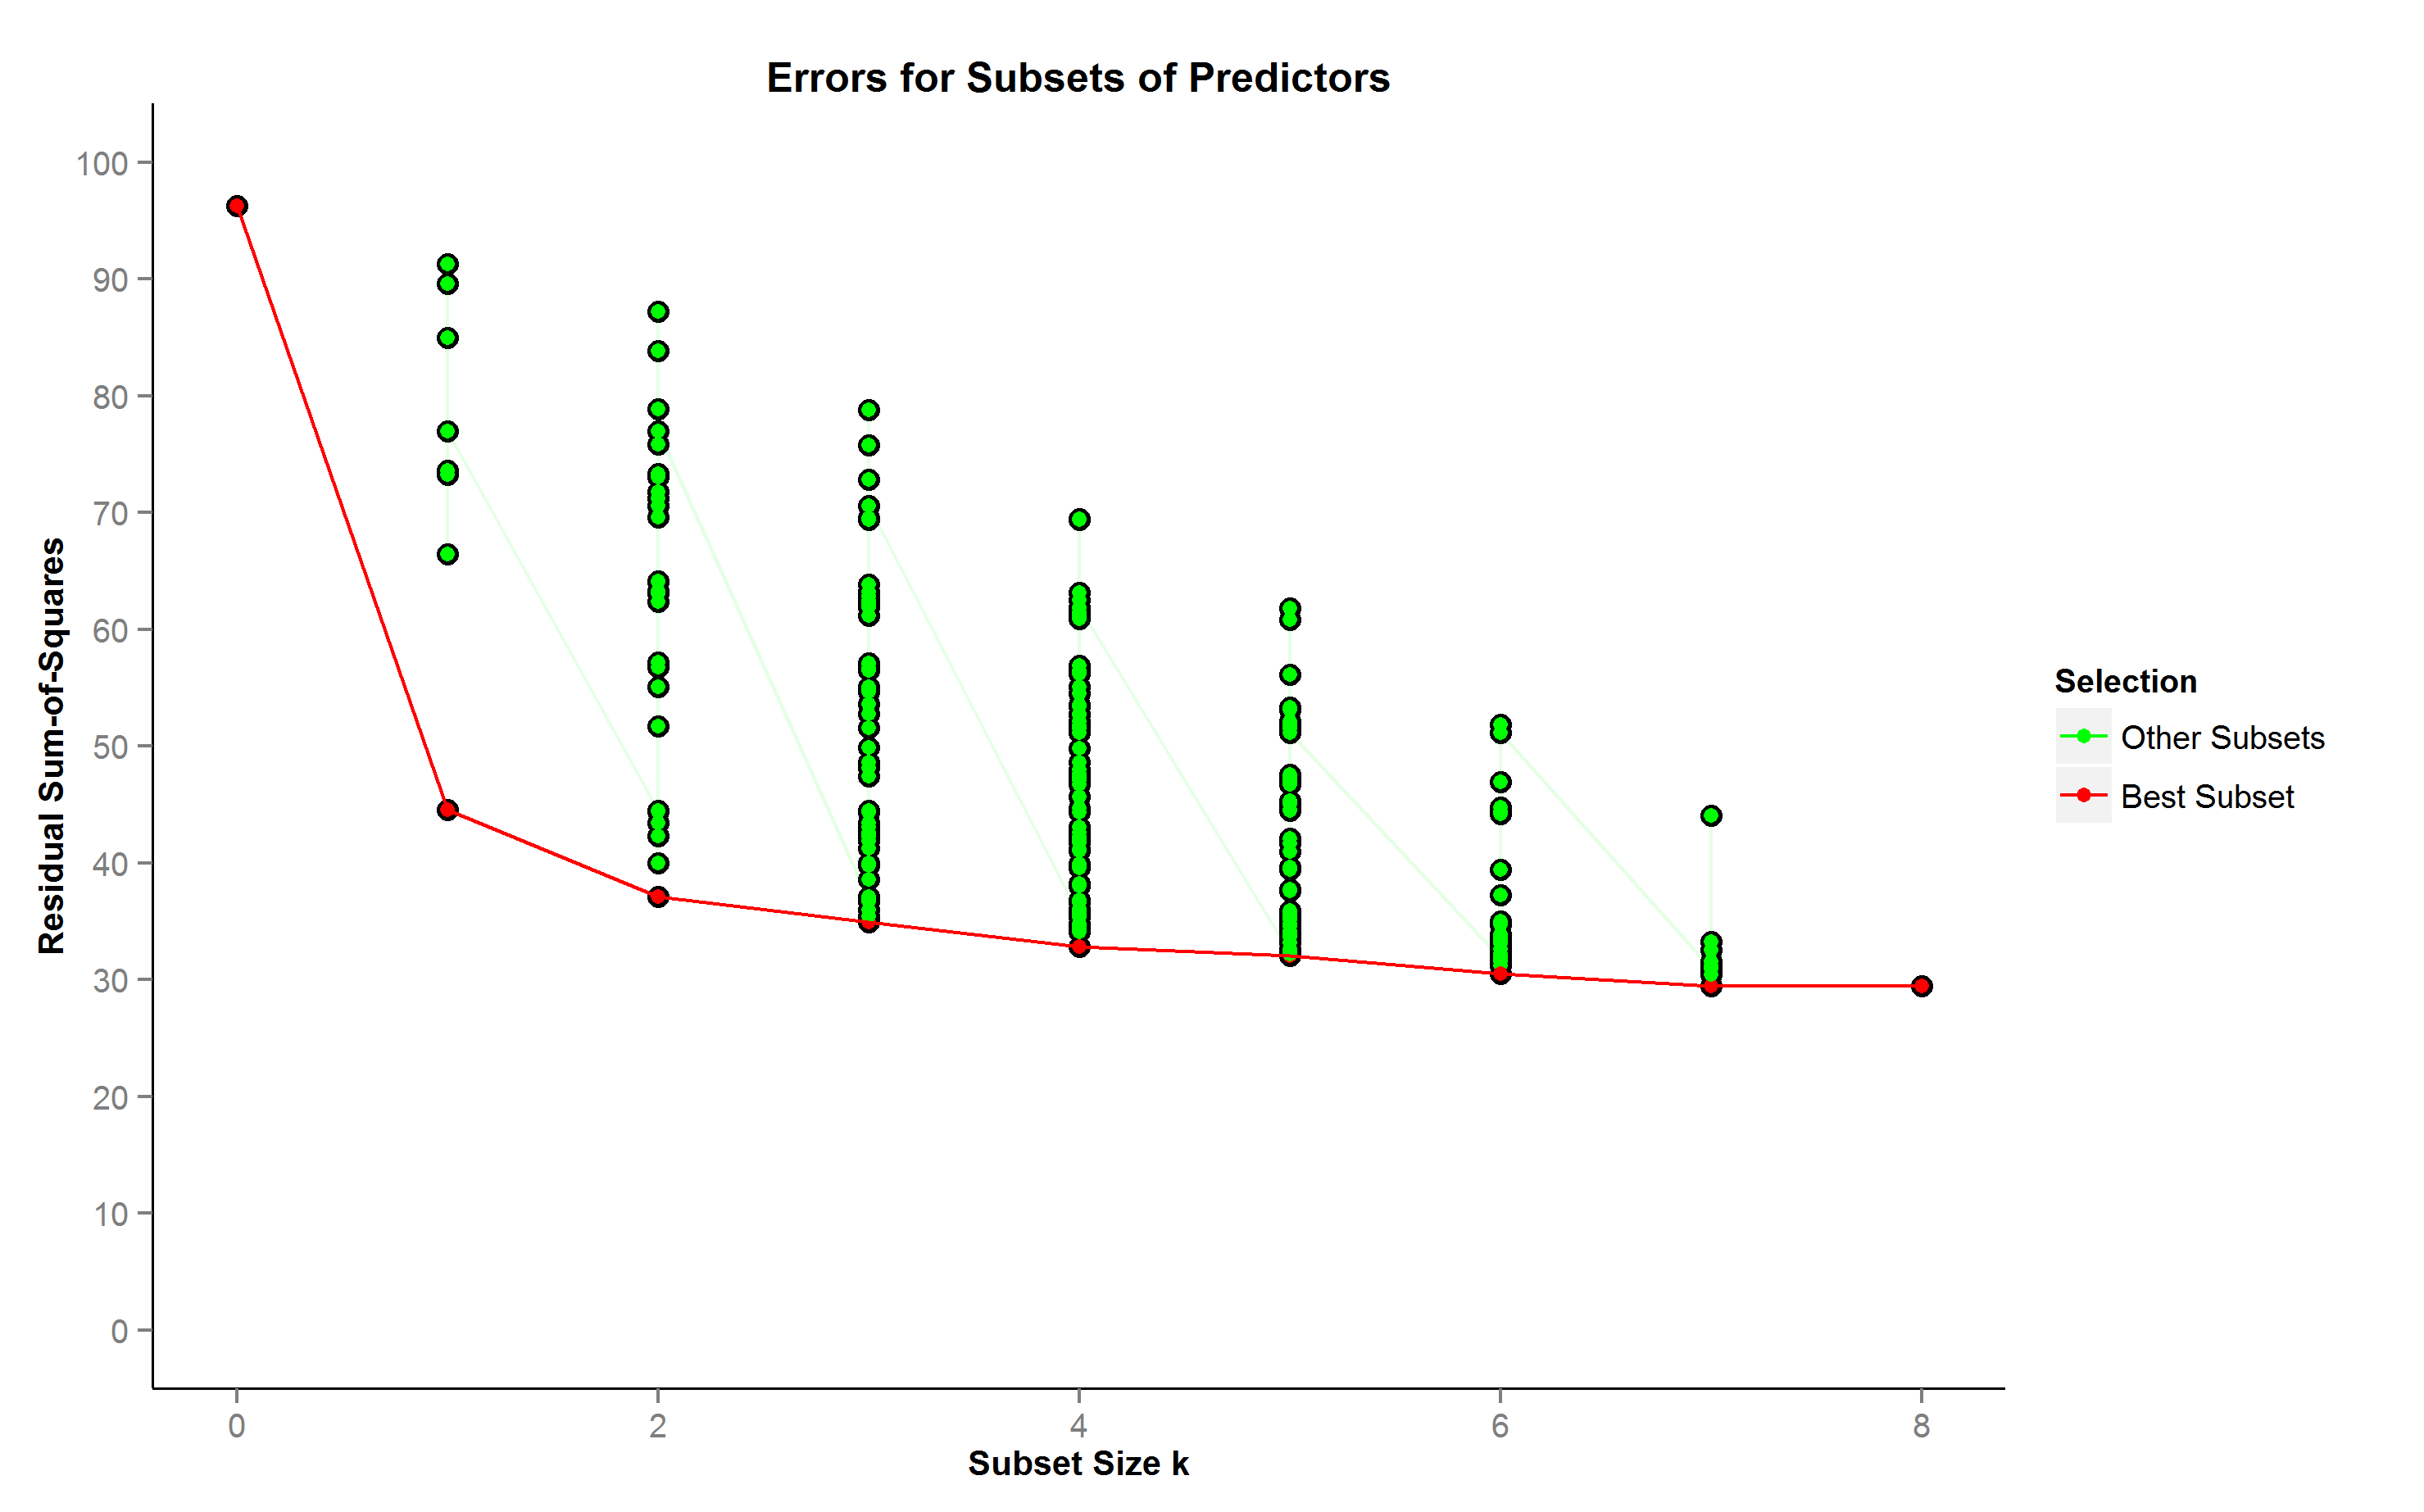
\includegraphics[width=.8\linewidth]{HW03_Exercise01}
    \caption{An error plot for all subsets of features for the prostate cancer data set.}
    \label{fig:HW03_Exercise01}
  \end{figure}

\subsection{Code}
The following R code was used to reproduce the figure from the book.
\begin{verbatim}
##################
# STAT775
# HW 03
# Exercise 01
#
# Reproduce Figure 3-5 from the
# Elements of Statistical Learning
# (This is a scatterplot of the
# errors produced by models built
# from all possible subsets of
# predictors, except for an
# intercept, for simplicity)
#
##################

#
# Initial Setup
#
setwd("C:/Users/Terence/Documents/GitHub/STAT775/HW03")
# setwd("~/STAT775/HW03/")

RESULTS.FILE.NAME = "HW03_Exercise01.png"
DATA.FILE.NAME <- "prostate_cancer/prostate_cancer_data"
# these include the intercept that gets added to the matrices
FEATURE.INDICES <- 1:9
TARGET.INDEX <- 10
TRAIN.SET.FLAG <- 11


data <- read.table(DATA.FILE.NAME)
# according to the dataset info, this needs to be done
data[, 1:8] <- scale(data[, 1:8], T, T)
intercept <- rep(1, nrow(data))
data <- data.frame(Intercept = intercept, data)


# store data with rows as observations
train.data <- data.matrix(subset(data, data$train == T))[, FEATURE.INDICES]
train.targets <- data.matrix(subset(data, data$train == T))[, TARGET.INDEX]
test.data <- data.matrix(subset(data, data$train == F))[, FEATURE.INDICES]
test.targets <- data.matrix(subset(data, data$train == F))[, TARGET.INDEX]


#
# Regression
#
model.betas <-
  solve(t(train.data) %*% train.data) %*% t(train.data) %*% train.targets


#
# Test errors
#
feature.subsets <- set_power(as.set(2:9))  # skip excluding intercept

k <- rep(0, length(feature.subsets))
subset.as.string <- rep("", length(feature.subsets))
error <- rep(0, length(feature.subsets))
best.for.k <- rep(F, length(feature.subsets))

subset.selection.results <- data.frame(
  K = k,
  Subset = subset.as.string,
  Error = error,
  Best.For.K = best.for.k,
  stringsAsFactors = F
)

index = 1
residual.sum.of.squares <- 0
for (subset in feature.subsets) {
  subset.betas <- matrix(rep(0, 9))
  subset.betas[1, ] <- model.betas[1, ]
  for (i in subset) {
    subset.betas[i, ] <- model.betas[i, ]
  }
  
  # do the eror test here
  residual.sum.of.squares <- 0.0
  for (i in 1:nrow(train.data)) {
    prediction <- t(subset.betas) %*% data.matrix(train.data[i, ])
    residual.sum.of.squares <-
      residual.sum.of.squares + (train.targets[i] - prediction)^2
  }
  
  # append the results
  subset.selection.results$K[[index]] <- length(subset)
  subset.selection.results$Subset[[index]] <-
    if(set_is_empty(subset)){"Empty"} else{subset}
  # str_c(list, collapse = ',') or paste(list, collapse = ',')
  subset.selection.results$Error[[index]] <- residual.sum.of.squares
  index = index + 1
}

subset.selection.results$K <- as.factor(subset.selection.results$K)

for (level in levels(subset.selection.results$K)) {
  print(level)
  working.set <-
    subset(subset.selection.results, subset.selection.results$K == level)
  working.set <- working.set[order(working.set$Error), ]
  best.subset <- working.set[1, "Subset"]
  print(best.subset)
  i=1
  for (i in nrow(subset.selection.results)) {
    if (set_is_equal(best.subset, subset.selection.results[i, "Subset"])) {
      subset.selection.results$Best.For.K[[i]] <- T
    }
  }
}

# have to do this manually because R sux #########
subset.selection.results[  1, "Best.For.K"] <- T
subset.selection.results[  2, "Best.For.K"] <- T
subset.selection.results[ 10, "Best.For.K"] <- T
subset.selection.results[ 40, "Best.For.K"] <- T
subset.selection.results[ 99, "Best.For.K"] <- T
subset.selection.results[181, "Best.For.K"] <- T
subset.selection.results[231, "Best.For.K"] <- T
subset.selection.results[249, "Best.For.K"] <- T
subset.selection.results[256, "Best.For.K"] <- T
##################################################


#
# Plot Results
#
library(ggplot2)

plot.theme <- theme(
  plot.background = element_blank(), 
  panel.grid.major = element_blank(), 
  panel.grid.minor = element_blank(), 
  panel.border = element_blank(), 
  panel.background = element_blank(),
  axis.line = element_line(size=.4),
  axis.title.x = element_text(face="bold", color="black", size=10),
  axis.title.y = element_text(face="bold", color="black", size=10),
  plot.title = element_text(face="bold", color = "black", size=12)
)

subset.error.plot <- ggplot(
  subset.selection.results,
  aes(x = K, y = Error, group = Best.For.K)
) +
  plot.theme +
  geom_point(shape = 16, size = 3) +
  geom_point(aes(color = Best.For.K)) +
  geom_line(aes(alpha = Best.For.K, color = Best.For.K)) +
  scale_color_manual(
    name = "Selection",
    labels = c("Other Subsets", "Best Subset"),
    values = c("green", "red")
  ) +
  scale_shape_manual(
    name = "Selection",
    labels = c("Other Subsets", "Best Subset"),
    values = c(16, 8)
  ) +
  scale_alpha_discrete(guide = F) + #continuous
  scale_y_continuous(
    limits = c(0, 140),
    breaks = seq(0, 140, 10)
  ) +
  labs(
    title = "Errors for Subsets of Predictors",
    x = "Subset Size k",
    y = "Residual Sum-of-Squares"
  )

ggsave(filename = RESULTS.FILE.NAME, plot = subset.error.plot)
\end{verbatim}

\newpage
\section{Ridge Regression}
\subsection{Problem Description}
Apply the Ridge Regression Technique to the prostate cancer data. Plot the error results as a function of $\lambda$. The choice of $\lambda$ values is up to you.

\subsection{Results}
  \begin{figure}[h!]
    \centering
    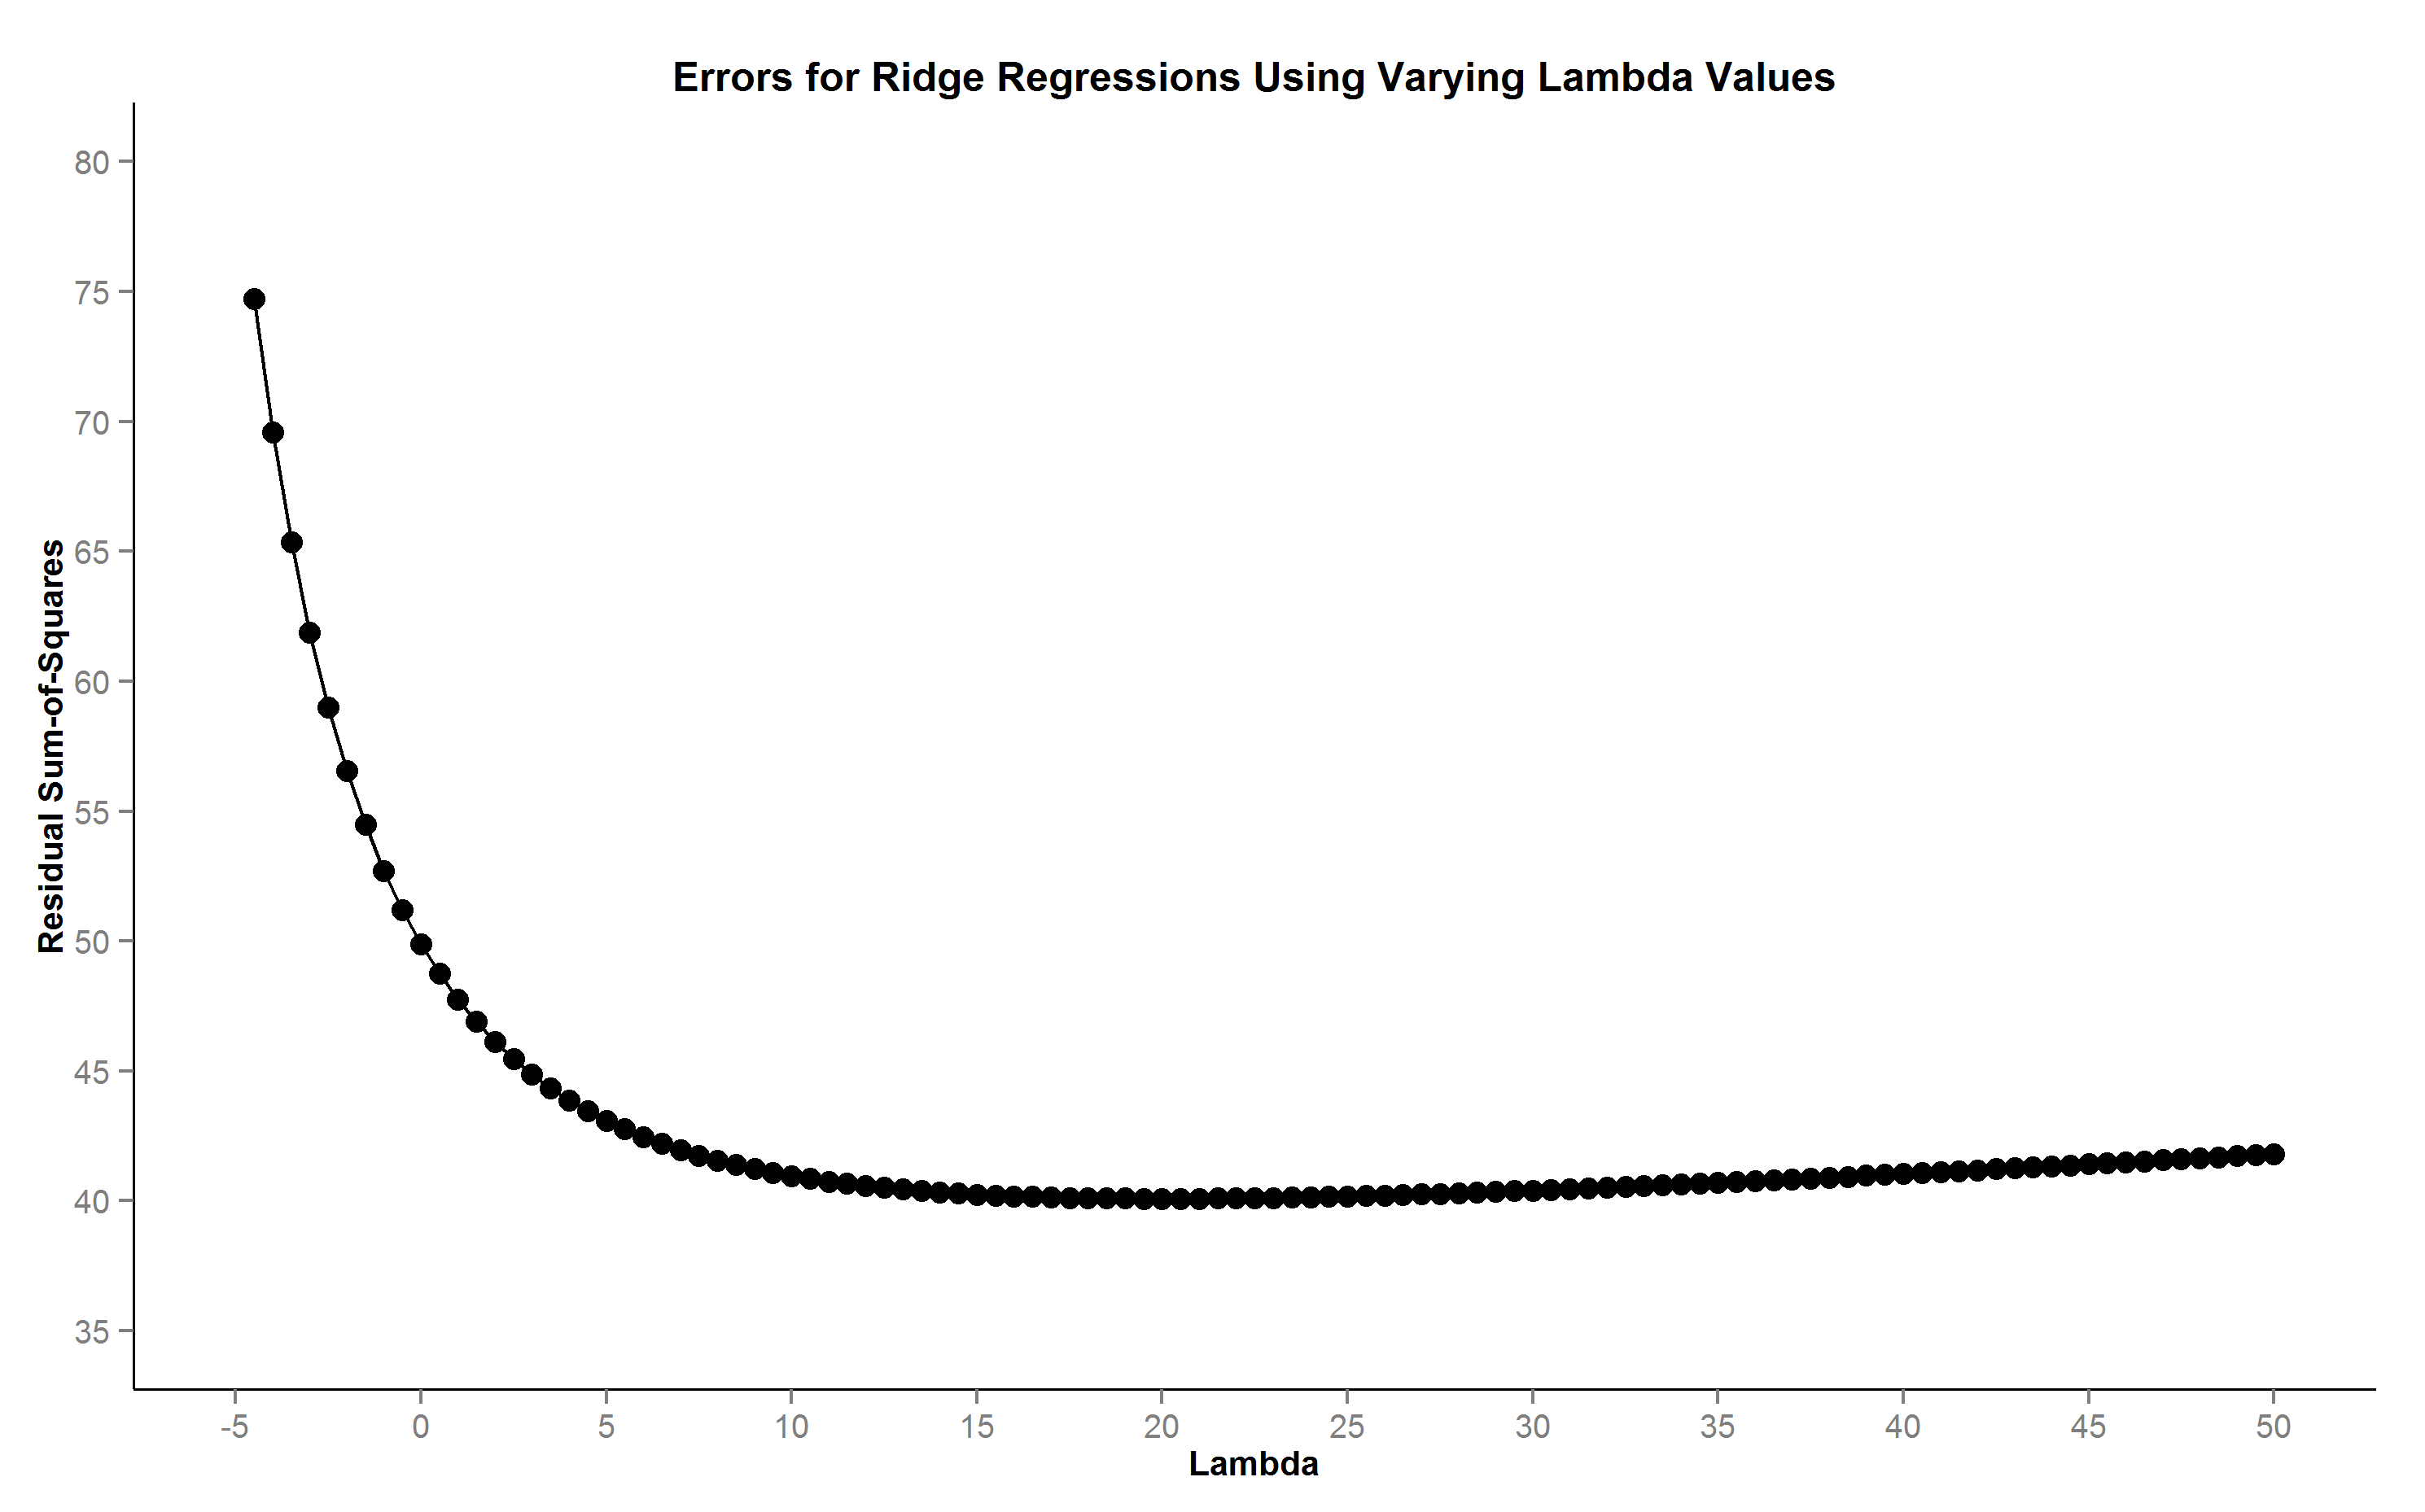
\includegraphics[width=.8\linewidth]{HW03_Exercise02}
    \caption{An error plot for Ridge Regression of the prostate cancer data with varying values of the parameter $\lambda$.}
    \label{fig:HW03_Exercise02}
  \end{figure}

\subsection{Code}
\begin{verbatim}
##################
# STAT775
# HW 03
# Exercise 02
#
# Perform Ridge Regression
# and explore the performance
# of using different
# lambda values. Plot the
# results.
#
##################

#
# Initial Setup
#
setwd("C:/Users/Terence/Documents/GitHub/STAT775/HW03")
# setwd("~/STAT775/HW03/")

RESULTS.FILE.NAME = "HW03_Exercise02.png"
DATA.FILE.NAME <- "../DataSets/prostate_cancer/prostate_cancer_data"
# no intercept will be applied since we are performing
# ridge regression
FEATURE.INDICES <- 1:8
TARGET.INDEX <- 9
TRAIN.SET.FLAG <- 10

data <- read.table(DATA.FILE.NAME)
# according to the dataset info, this needs to be done
data[, FEATURE.INDICES] <- scale(data[, FEATURE.INDICES], center = T, scale = T)

# store data with rows as observations
train.data <- data.matrix(subset(data, data$train == T))[, FEATURE.INDICES]
intercepts <- rep(1, nrow(train.data))
train.data.with.intercepts <- cbind(intercepts, train.data)
train.targets <- data.matrix(subset(data, data$train == T))[, TARGET.INDEX]

test.data <- data.matrix(subset(data, data$train == F))[, FEATURE.INDICES]
intercepts <- rep(1, nrow(test.data))
test.data.with.intercepts <- cbind(intercepts, test.data)
test.targets <- data.matrix(subset(data, data$train == F))[, TARGET.INDEX]


#
# Ridge Regression
#
ridge.regression <- function(x, y, lambda) {
 #
 # Args:
 #   x: a matrix of training observations where observations are rows
 #   y: a column vector of regression targets
 #   lamba: the ridge coefficient; larger values reduce the effect of less
 #          relevant features

  lambda.I <- diag(lambda, nrow = ncol(x))
  model.betas <- solve( (t(x) %*% x) + lambda.I) %*% t(x) %*% y
  model.betas <- rbind(mean(y), model.betas)

  return(list(
    beta.hat = matrix(model.betas, nrow = 1)
  ))
}

predict <- function(model, x) {
  #
  # Args:
  #   model: an n x 1 column vector of regression coefficients
  #   x: a ? x n matrix of observation data

  return(model$beta.hat %*% t(x))
}

#
# Main
#
lambda.values <- seq(from = 0, to = 8, by = .5)
ridge.regression.results <- data.frame(
  row.names = lapply(as.list(lambda.values), toString),
  'Lambda' = lambda.values,
  'RSS' = rep(0, length(lambda.values)),
  stringsAsFactors = F
)

trial <- 1
for (lambda in lambda.values) {
   model <- ridge.regression(x = train.data, y = train.targets, lambda = lambda)
#   model <- list(beta.hat = matrix(c(2.452, 0.42, 0.238, -0.046, 0.162, 0.227, 0.000, 0.040, 0.133), nrow = 1))
  predictions <- predict(model, cbind(1, train.data))

  ridge.regression.results[toString(lambda), 'RSS'] <-
    sum((matrix(train.targets, nrow = 1) - predictions) ^ 2)
}

#
# Plot Results
#
library(ggplot2)

plot.theme <- theme(
  plot.background = element_blank(),
  panel.grid.major = element_blank(),
  panel.grid.minor = element_blank(),
  panel.border = element_blank(),
  panel.background = element_blank(),
  axis.line = element_line(size=.4),
  axis.title.x = element_text(face="bold", color="black", size=10),
  axis.title.y = element_text(face="bold", color="black", size=10),
  plot.title = element_text(face="bold", color = "black", size=12)
)

error.plot <- ggplot(
  ridge.regression.results,
  aes(x = Lambda, y = RSS)
) +
  plot.theme +
  geom_point(shape = 16, size = 3) +
  geom_line() +
  scale_x_continuous(
    limits = c(-5, 50),
    breaks = seq(-5, 50, 5)
  ) +
  scale_y_continuous(
    limits = c(35, 80),
    breaks = seq(35, 80, 5)
  ) +
  labs(
    title = "Errors for Ridge Regressions Using Varying Lambda Values",
    x = "Lambda",
    y = "Residual Sum-of-Squares"
  )
error.plot

ggsave(filename = RESULTS.FILE.NAME, plot = error.plot)
\end{verbatim}

\newpage
\section{Principle Component Analysis}
\subsection{Problem Description}
Use the zipcode digit data from the ESL website, repeat the exercise from HW02 (Na\"{i}ve Bayes Classification), but this time use the $16$ best ``Eigen-features", aka principle components, (or as many as you can if $16$ eigen-vectors do not exist for the data) for classification instead of the $256$ pixel value features.

\subsection{Results}
It might be said that using the principle components performed worse than naive Bayes classification, but only 16 principle component features were used, meaning some information was lost. Perhaps finding an ideal number of principle components or using enough to encode some high percentage of the information would give us extremely good classification results. The confusion matrix below details the classification performance:

\begin{tabular}{| c || c | c | c | c | c | c | c | c | c | c | c |}
  \hline
  Actual/Prediction &   0 &   1 &   2 &   3 &   4 &   5 &   6 &   7 &   8 &   9 &\% Correct \\
  \hline
  \hline
  0                 & 344 &   0 &   5 &   0 &   1 &   3 &   3 &   0 &   2 &   1 & 95.8 \\
  \hline
  1                 &   0 & 241 &   2 &   0 &   8 &   1 &   5 &   0 &   6 &   1 & 91.3 \\
  \hline
  2                 &   4 &   0 & 182 &   2 &   1 &   6 &   0 &   0 &   3 &   0 & 91.9 \\
  \hline
  3                 &   1 &   0 &   2 & 143 &   0 &  15 &   0 &   1 &   4 &   0 & 86.1 \\
  \hline
  4                 &   0 &   1 &  10 &   0 & 181 &   2 &   0 &   0 &   0 &   6 & 90.5 \\
  \hline
  5                 &   1 &   0 &   0 &   7 &   1 & 144 &   0 &   0 &   4 &   3 & 90.0 \\
  \hline
  6                 &   0 &   0 &   3 &   0 &   3 &   4 & 158 &   0 &   2 &   0 & 92.9 \\
  \hline
  7                 &   0 &   0 &   4 &   0 &   2 &   4 &   0 & 130 &   4 &   3 & 88.4 \\
  \hline
  0                 &   1 &   0 &   3 &   7 &   0 &   6 &   0 &   0 & 150 &   4 & 90.4 \\
  \hline
  0                 &   0 &   0 &   2 &   1 &   4 &   0 &   0 &   2 &   6 & 162 & 91.5 \\
  \hline
  \hline
  Overall           & & & & & & & & & &                                         & 91.43 \\
  \hline
\end{tabular}

\subsection{Code}
The following R code was used to solve the classification problem:
\begin{verbatim}
setwd("C:/Users/Terence/Documents/GitHub/STAT775/HW06")

DATA.PATH <- "../DataSets/zip.data/"
ZIP.TRAIN.FILE.NAME <- paste0(DATA.PATH, "zip.train")
ZIP.TEST.FILE.NAME <- paste0(DATA.PATH, "zip.test")


read.data.tuples <- function(file.path.name) {
  data.fram.e <- read.table(file.path.name)

  data <- data.matrix(data.fram.e[, -1])

  data.tuple <- list(
    observations = data,
    labels = data.matrix(data.fram.e[, 1])
  )
  return(data.tuple)
}

#
# PCA
#

get.pca.summary <- function(data, num.components = 20) {
  #
  # Args:
  #   data: an n x m matrix of n observations of m dimensions
  #   num.components: the number of principle components to keep

  num.component.s <- min(ncol(data), num.components)
  n.obs <- nrow(data)
  full.dimensionality <- ncol(data)
  mu <- colMeans(data)

  # get centered data
  x <- data
  for (i in 1:n.obs) {
    x[i, ] <- data[i, ] - mu
  }

  # covariance matrix
  sigma <- t(x) %*% x
  sigma <- sigma * (1.0 / n.obs)

  eigen.decomposition <- eigen(sigma, F)  # TODO: is cov symmetric? Not sure...
  eigen.vectors <- eigen.decomposition$vectors[, 1:num.component.s]

  pca.summary <- list(
    rotation = eigen.vectors,
    mu = matrix(mu, nrow = 1, ncol = full.dimensionality)
  )

  return(pca.summary)
}

predict <- function(pca.summary, data) {
  #
  # Args:
  #   data: an n x d matrix of observations; rows are observations
  #   pca.summary: a tuple of the rotation matrix (eigenvectors as columns) and
  #                the mean (row vector of column means) computed in the pca
  #                computations

  x <- data
  for (i in 1:nrow(data)) {
    x[i, ] <- data[i, ] - pca.summary$mu
  }

  return (t(t(pca.summary$rotation) %*% t(x)))
}


train <- read.data.tuples(ZIP.TRAIN.FILE.NAME)

pca.model <- get.pca.summary(train$observations, 16)

train$observations <- predict(pca.model, train$observations)

train.frame <- data.frame('class' = train$labels, train$observations)

CLASSES <- list(0,1,2,3,4,5,6,7,8,9)
class.summaries <- list(10)
for (k in CLASSES) {
  data.subset <- subset(train.frame, class == k)
  n <- nrow(data.subset)
  mu <- colMeans(data.subset[, -1])
  sigma <- cov(data.subset[, -1])
  class.summaries[[k + 1]] <- list(
    label = k,
    n = n,
    mu = mu,
    sigma = sigma
  )
}

gaussian.pdf <- function(k, x) {
  x <- matrix(x, ncol = 1)
  scale.f <- 1.0 / sqrt(((2.0 * pi) ^ 16) * det(k$sigma))
  difference <- x - matrix(k$mu, ncol = 1)
  exponent <- -0.5 * (t(difference) %*% solve(k$sigma) %*% difference)
  return(scale.f * exp(exponent))
}

classify.object <- function(classes, x) {
  highest.prob <- 0.0
  most.probable.class.label <- 0
  for (i in 1:length(classes)) {
    prob <- gaussian.pdf(k = classes[[i]], x = x) * classes[[i]]$n
    if (prob > highest.prob) {
      highest.prob <- prob
      most.probable.class.label <- classes[[i]]$label
    }
  }

  return(most.probable.class.label)
}

test <- read.data.tuples(ZIP.TEST.FILE.NAME)
test$observations <- as.matrix(predict(pca.model, test$observations))
test$observations <- matrix(
  test$observations[, 1:16],
  nrow = nrow(test$observations),
  ncol = 16
)

num.correct <- 0
confusion.matrix <- matrix(0, nrow = 10, ncol = 11)
for (i in 1:nrow(test$labels)) {
  prediction <- classify.object(class.summaries, x = test$observations[i, ])
  if (prediction == test$labels[[i]]) {
    num.correct <- num.correct + 1
  }

  confusion.matrix[test$labels[[i]] + 1, prediction + 1] <-
    confusion.matrix[test$labels[[i]] + 1, prediction + 1] + 1

}

totals <- rowSums(confusion.matrix)
for (i in 1:nrow(confusion.matrix)) {
  confusion.matrix[i, 11] <- (confusion.matrix[i,i] / totals[[i]]) * 100
}


print(100 * num.correct / nrow(test$labels))
print(confusion.matrix)
\end{verbatim}

\section{The student would like to thank...}
The student would like to thank the authors of the Eigen C++ matrix library. This library has proved quick, easy and effective numerous times, this time being no exception. The Eigen library and more information can both be found at\hfill\\
\texttt{http://eigen.tuxfamily.org}.

\end{document}
